%pdflatex -halt-on-error -aux-directory=tmp -output-directory=tmp rapport.tex%

\documentclass{article}
\usepackage{amsmath}
\usepackage[utf8]{inputenc}
\usepackage[T1]{fontenc}
\usepackage{graphicx}
\usepackage{hyperref}
\usepackage[francais]{babel}
\usepackage{listings}
\usepackage{xcolor}

\definecolor{codegreen}{rgb}{0,0.6,0}
\definecolor{codegray}{rgb}{0.5,0.5,0.5}
\definecolor{codepurple}{rgb}{0.58,0,0.82}
\definecolor{backcolour}{rgb}{0.95,0.95,0.92}

\lstdefinestyle{mystyle}{
    language=python,
    backgroundcolor=\color{backcolour},   
    commentstyle=\color{codegreen},
    keywordstyle=\color{magenta},
    numberstyle=\tiny\color{codegray},
    stringstyle=\color{codepurple},
    basicstyle=\ttfamily\footnotesize,
    breakatwhitespace=false,         
    breaklines=true,                 
    captionpos=b,                    
    keepspaces=true,                 
    numbers=left,                    
    numbersep=5pt,                  
    showspaces=false,                
    showstringspaces=false,
    showtabs=false,                  
    tabsize=2
}

\lstset{style=mystyle}

\title{Théorie des langages II}
\author{Wassim SAIDANE}
\date{12/03/2021}

\begin{document}
    \pagenumbering{gobble}
    \maketitle
    \pagenumbering{arabic}
    \section*{Note : }
    Ce cours est ma prise de note du cours de L3 infos de Théorie des langages II de Mamadou Kante
    \section*{Chapitre 2 : Automates à pile (non terminé)}
    L'objectif de ce chapitre est de montrer que une correspondance entre grammaires algébriqus et automates à pile. \\
    \\
    Un automate à pile est un automate à états finis muni d'une pile. A chaque étape, l'état suivant est détérminé par l'état courant, la lettre $u$ et l'état de la pile. \\
    \\
    \underline{Définition 2.1} Un automate à pile est un tuple $A=(Q, \Sigma, \Gamma, \delta, q_0, F)$ tel que : 
    \begin{enumerate}
        \item $Q$ est un ensemble fini, appelé ensemble des états. 
        \item $\Sigma$ : Est un ensemble fini, alphabet des mots à reconnaitre. 
        \item $\Gamma$ : Ensemble fini, alphabet de la pile. 
        \item $\delta$ : $Q \times (\Sigma \bigcup \{\epsilon\}) \times (\Gamma \bigcup \{\epsilon\}) \rightarrow 2^{Q \times (\Gamma \bigcup \{\epsilon\})}$
        \item $q_0 \in Q : $Etat initial. 
        \item $F \subseteq Q :$ Etats finaux 
    \end{enumerate}
    \underline{Exécutions d'un automate à pile}
    Une exécution accptante d'un mot $w \in \Sigma^R$ par $A$: Si on peut récrire $w$ en $w_1,w_2,w_3,..,w_m$, où $w_i \in \Sigma \bigcup \{\epsilon\}$ (on ajoute des $\sigma$ entre les lettres de $w$) et si on a une séquance d'états $r_0,r_1,...,r_m$ et de mots $s_0,s_1,s_2,..,s_m \in \Gamma^*$ tels que : \\
    \begin{enumerate}
        \item $r_0=q_0$, $s_0=\epsilon$ (on commence par l'état initial et une pile vide)
        \item $\forall 0 \le i \le m-1, (r_{i+1},b) \in \delta (r_i, w_{i+1}, a)$ où $s_i=at, s_{i+1}=bt, a,b \in \Gamma \bigcup \{\epsilon\} t \in \Gamma^*$ \\
        Si on est à l'état $r_i$, on lit la lettre $w_{i+1}$ (qui peut être la lettre $\epsilon$), la tête de la pile c'est $a$(ou $\epsilon$), on passe à l'état $r_{i+1}$, on empile la lettre $b$ dans la pile ($b$ peut être vide, signifiant on n'empile rien). \\
        \item $r_m \in F$
    \end{enumerate}
    Le langage de $A$, noté $L(A)$, l'ensemble des mots $w$ tel que il existe une exécution acceptante de $A$ sur $w$. \\
    Comme pour les automates à états finis, on peut donner un automate avec un dessin (représentation visuelle) : Graphe orienté avec sommets les états, et les arcs sont étiqutés par les transitions : \\ 
    La lettre à lire, la tête de la pile et l'opération à faire sur la pile. \\
    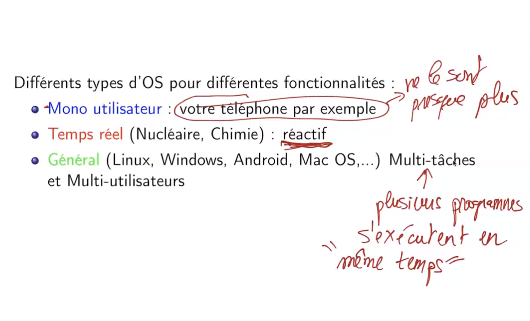
\includegraphics{capture/5.PNG}
    \underline{Exemple : } \\
    $L=\{0^n1^n \mid n \ge 1\}$ \\
    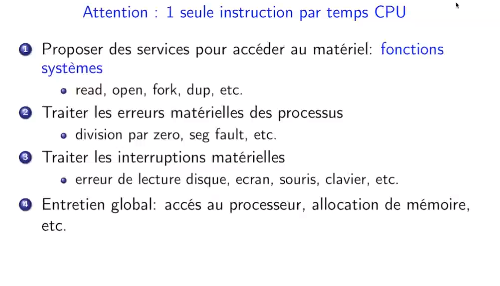
\includegraphics{capture/6.PNG} \\ 
    \newpage
    $0,\varepsilon \rightarrow 0 : $ Je ne sépile rien, jempile 0 \\ 
    $1,0 \rightarrow \varepsilon : $ Je dépile et je n'empile rien \\ 
    $a \in \Sigma$ $b,c \in \Gamma$ (tous différents de $\varepsilon$) \\ 
    $a,b \rightarrow c$ : Si je lis a, la tête de pile c'est b, je dépile b et j'empile c. \\ 
    $a, \varepsilon \rightarrow c : $ Si je lis a, j'empile c \\ 
    ($\varepsilon, \varepsilon \rightarrow \$ : $ Je ne lis rien, j'empile \$) \\ 
    $a,b \rightarrow \varepsilon : $ Si je lis a, la tête de pile c'est b, je dépile \\ 
    \\
    \underline{Théorème 2.1 :} Un langage $L \subseteq \Sigma^*$ est algébrique $\Leftrightarrow$ il existe un automate à pile $A$ tel que $L=(A)$. \\ 
    \underline{Cas particulier :} \\ 
    \begin{enumerate}
        \item On voit que tout automate à états finis estun automate à pile (on oublie la pile dans les transitions). \\ 
        \item Toute expression régulière est un cas particulier d'une grammaire hors contexte.
        $r=a : $ $s \rightarrow a$ \\
        $r=r_1 \cdot r_2 :$ $S_i : $ La variable de départ de $G_1$ qui est la grammaire aglébrique décrivant $r_i$ et donc on vérifie que : $S \rightarrow S_1S_2$ \\ 
        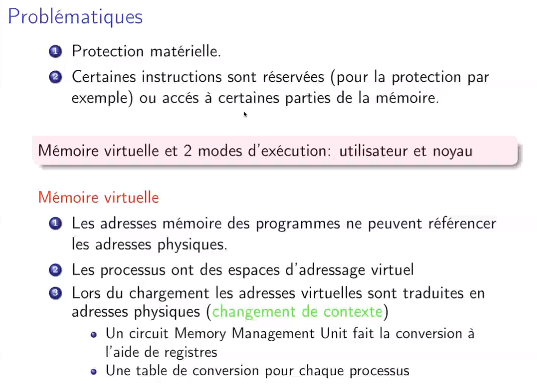
\includegraphics{capture/7.PNG} \\
        \item Pareil si $r=r_1+r_2$ \\ 
        $S \rightarrow S_1 \mid S_2$ \\
        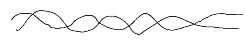
\includegraphics{capture/8.PNG}
        \item Si $r=s^* :$ $G$ la grammaire décrivant $S$, avec $S$ la variable de départ, la grammaire algébrique par $r$ : \\ 
        \begin{equation*}
            T \rightarrow \varepsilon \mid ST
        \end{equation*}
        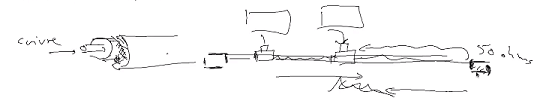
\includegraphics{capture/9.PNG}
        \begin{equation*}
            T \Rightarrow ST \Rightarrow SST \Rightarrow SSST \Rightarrow SSS\epsilon
        \end{equation*}
        (on aura répété trois fois l'expression rationnelle $S$) \\ 
        \underline{Preuve $\Rightarrow$}
        $L$ horst contexte $\Rightarrow L=L(A), A$ automate à pile. \\ 
        $L$ hors contexte : $\exists$ une grammaire horst contexte $G$ tel que $L=L(G)$. L'automate à pile $A$ va simuler la dérivation d'une mot : \\
        L'automate commence par empiler la variable de départ $S$. Ensuite, essayez chacun des mots que l'on peut dériver depuis $S$, en l'empilant. Et on fait pareil pour chacune des variables. \\ 
        Les transitions sont : \\ 
        \begin{itemize}
            \item Au départ on empile $\$$ (pur détecter que l'on a tout dépiler : Détecter une pile vide). Ensuite on empile $S$. [Au départ on a : $S\$$].
            \item Si $A$ est la tête de la pile et $A \rightarrow w$ est une règle, on a la transition qui dépile $A$ et empile les lettres de $w=w_1w_2,...w_p$ dans l'ordre $w_p,w_{p-1},...,w_i$ [w_1 sera la tête de pile].
            \item Si $a \in \Sigma$ est la tête de pile, a est la lettre lue dans le mot, on dépile [on avance dans la lecture du mot]. \\
            On peut montrer sans difficulté (par induction) que $A$ accepte $w$ ssi $S \Rightarrow^* w$\\
        \end{itemize}
        \underline{Preuve $\Leftarrow$} 
        $L=L(A)$ pur un automate à pile, alors il existe une grammaire hors contexte $G$ telle que $L=L(G)$. \\
        La preuve est su même type que celle qui montre que tout langage reconnaissable est rationnel. \\
        On va commencer par simplifier l'automate : \\ 
        \begin{itemize}
            \item Il n'a qu'un seul état final, $q_B$
            \item Il vide la pile, avant d'accepter
            \item chaque transition ne fait qu'un seule opération sur la pile : soit elle empile (et ne dépile pas), soit elle dépile (mais n'empile pas). \\
        \end{itemize}
        Maintenant, on note $L_{p,q} : $ L'ensemble des mots que je peux lire depuis l'état $p$(avec pile vide) et terminer sur l'état $q$ (avec pile vide). \\
        Avec la modification il n'y a qu'un seul état final $q_f$, on a : 
        \begin{equation*}
            L_{q_0,q_f}=L(A)    
        \end{equation*}
        Les variables seront : $L_{q,q'}, q,q' \in Q$ \\
        Par exemple si on lit $w$ depuis l'état $p$ (avec pile vide), on arrive à l'étatt $q$ (avec pile vide) et on continue la lecture de $w$ et termine sur $q'$ (avec pile vide), alors $L_{p,q'} \rightarrow L_{p,q}L_{q,q'}$ \\
        On peut avoir également un comportement suivant dans l'automate : La lettre empilée au départ de la lecture de $w$, est celle dépilée à la fin de la lecture de $w$. \\ 
        Si on lisant $a$ depuis $p$, on empile $x$, on passe à l'état$r$, on continue la lecture de $w$ à l'état avec tête de pile =$x$ et on dépile $x$ lorsque l'on lit la dernière lettre de $w$ depuis l'état $s$, et ensuite on dépile $x$, alors on la règle $L_{p,q} \rightarrow aL_{r,s}b$ \\
        Si $w=aw_2 ... ,w_p b$ : \\
        L'automate a lu $a$, a empilé $x$, est passé à l'état $r$, a lu $w_2,...,w_p$, estarrivé à l'état $s$ et avec tete de pile =$x$ (sans jamais le dépiler dans la lecture de $w_2,...,w_^p$), et spuis $s$ est arrivé à l'état en dépilant $x$ et en lisant $b$. \\
        On ajoute les règles : $L_{p,p} \rightarrow \varepsilon$ \\
        \underline{Pour résumer : } \\
        \begin{enumerate}
            \item $\forall p,q,r \in Q$, on ajoute la règle : $L_{p,q} \rightarrow L_{p,r}L_{r,q}$ \\
            \item $\forall p \leftarrow Q$, on ajoute $L_{p,p} \rightarrow \varepsilon$
            \item $\forall p,q,r,s \in Q, t \in \Gamma, a,b \in \Sigma \bigcup \{\varepsilon\}$ si $(r,t) \in \gramma(p,a,\varepsilon)$ et $(q, \varepsilon) \in \gamma(s,b,t)$, on ajoute la règle $L_{p,q} \rightarrow aL_{r,s}b$
        \end{enumerate}
        Tous ce qu'il faut faire ensuite c'est montrer par induction que $L_{p,q} \Rightarrow^* w \Leftrightarrow w \in L_{p,q}$ (on peut lire $w$ à partir de l'état $p$, la pile contenant $t \in \Gamma^*$, arrivé à l'état en ayant lu tout w, et laisser $t \in \gamma^*$ dans la pile). \\
        \\ 
        \underline{Est-ce que tous les langages sont des langages algébrique ?} \\
        Non \\
        \underline{Comment montrer qu'un langage est non algébrique ?} \\ 
        On peut utiliser le \textbf{lemme de l'étoile des langages algébriques} \\
        \\
        \underline{Lemme de l'étoile des langages algébriques : }
        Si $L \subseteq \Sigma^*$ est un langage hors contexte, alirs il existe un entier p (appelé toujours \textbf{longueur d'itération} du langage $L$) et pour tout mot $w$, avec $\mid w \mid \ge p, \existsu,v,x,y,z \in \Sigma^*$ tel que $w=uvxyz$ avec : \\ 
        \begin{enumerate}
            \item $\mid vy \mid > 0 $(Au moins $v$ ou $y \neq \varepsilon$) 
            \item $\mid vxy \mid \le p$ 
            \item $\forall i\ge 0, uv^ixy^iz \in L$
        \end{enumerate}
        \underline{Idée de preuve : } Si $\mid w \mid >$ taille de la grammaire, alors il existe une variable que l'on dérivera au moins deux fois. On regarde l'arbre de dérivation et ensuite on regarde cette variable utilisée deux fois dans l'arbre de dérivation. Pour obtenir la décomposition en uvxuz, on prend une longueur qui nous garentit que par cette variable, on a appliqué la même règle deux fois. On obtient quelque cose comme : \\
        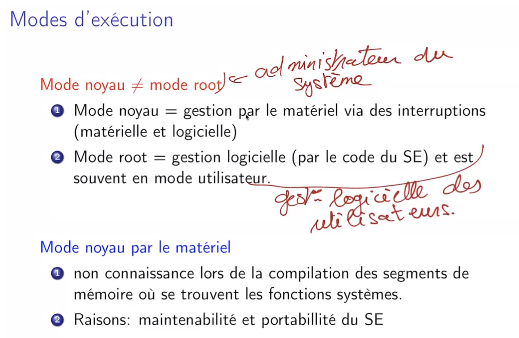
\includegraphics{capture/10.PNG} \\
        On la même règle applquée  deux fois : \\
        La 2ème application, si on regarde le sous arbre issu de la 2ème application, on obtient $x$ aux feuilles, la 1ère application de cette règle nous donne vxy aux feuilles, u est le préfixe et z le suffixe dans uvxyz. \\
        Si on prend la longueur de l'étoile = $b^{\mid V \mid +1}$, où b=longeur maximale d'un mot dérivé dans une règle : 
        \begin{equation*}
            b=\max \{\mid w : A \rightarrow w \text{est une règle} \}
        \end{equation*}
        On garantit qu'une règle est appliquéee deux fois au moins : La dernière utilisation donne $x$, l'avant dernière donne $vxy$.
        
    \end{enumerate}
\end{document}
